% copyright arturo salinas-aguayo 2025
\documentclass[12pt]{article}

\usepackage{graphicx}
\usepackage{subcaption}
\usepackage{amsmath}
\usepackage{siunitx}
\usepackage{array}
\usepackage{amsfonts}
\usepackage{fancyhdr}
\usepackage{geometry}
\usepackage{circuitikz}
\usepackage{caption}
\usepackage{bm}
\usepackage{float}

\geometry{letterpaper, margin=1in}
\graphicspath{ {../../images/} }

% Header and Footer
\pagestyle{fancy}
\fancyhf{}
\fancyhead[L]{ECE 2001 - Design Project 02: Audio Equalizer}
\fancyhead[R]{\thepage}
\setlength{\headheight}{15pt}

\author{Arturo Salinas-Aguayo}
\title{Design Project 02: Audio Equalizer}

% theorem set
\newtheorem{example}{Example}
% Example block environment
\newenvironment{examp}
{\vspace{0.5cm}
 \hrule
\vspace{0.5cm}
\begin{example}}
{\hrule
\vspace{0.5cm}
\end{example}}

\begin{document}
\newcommand{\closure}[2][3]{%
	{}\mkern#1mu\overline{\mkern-#1mu#2}}
\newcommand\ncoverline[1]{\mkern1mu\overline{\mkern-1mu#1\mkern-1mu}\mkern1mu}
% Title Page
\begin{titlepage}
	\centering
	\vspace*{3cm}
	\huge\textbf{Design Project 02: Audio Equalizer}\\

	\vspace{5cm}
	\Large\textbf{Arturo Salinas-Aguayo}\\
	\normalsize
	ECE 2001 Electrical Circuits\\
	Dr. David J. Giblin, Section 331.660.701.810-1253\\
	Mechanical Engineering Department
	\vfill
	
\includegraphics[scale=0.1]{uconnlogo}\\
	College of Engineering, University of Connecticut\\
	\scriptsize{Coded in \LaTeX}
	\vspace*{1cm}
\end{titlepage}
\tableofcontents
\newpage

\section{Abstract}
After being introduced to sinusoidal sources and reactive components in depth, the final project involves developing a more advanced music mixer that is capable of being tuned to attenuate or amplify certain frequencies.

There are many different applications when it comes to this vital tool, such as overboomy rooms at weddings, that leave speech muddy and unclear, to tuning a symphony hall's active speakers to bring out only the string instruments, without being too obvious that the instruments were indeed being amplified.

More recently, as cars have gotten better at dampening road noise and internal combustion engines are becoming smaller, companies such as GM and BMW are even tuning their sound systems to attempt to fool their customers that they are hearing the engine compared to a synthesized sound.

In practicality, this design project allows the opportunity to build on skills learned throughout the semester, starting with the build up on passive components, utilizing operational amplifiers, and then ending with the integration of reactive components such as inductors and capacitors.

\newpage
\section{Introduction}
Audio systems of days passed used to be synonymous with the graphic equalizer shown in Figure \ref{fig:equalizer}.

\begin{figure}[H]
	\centering
	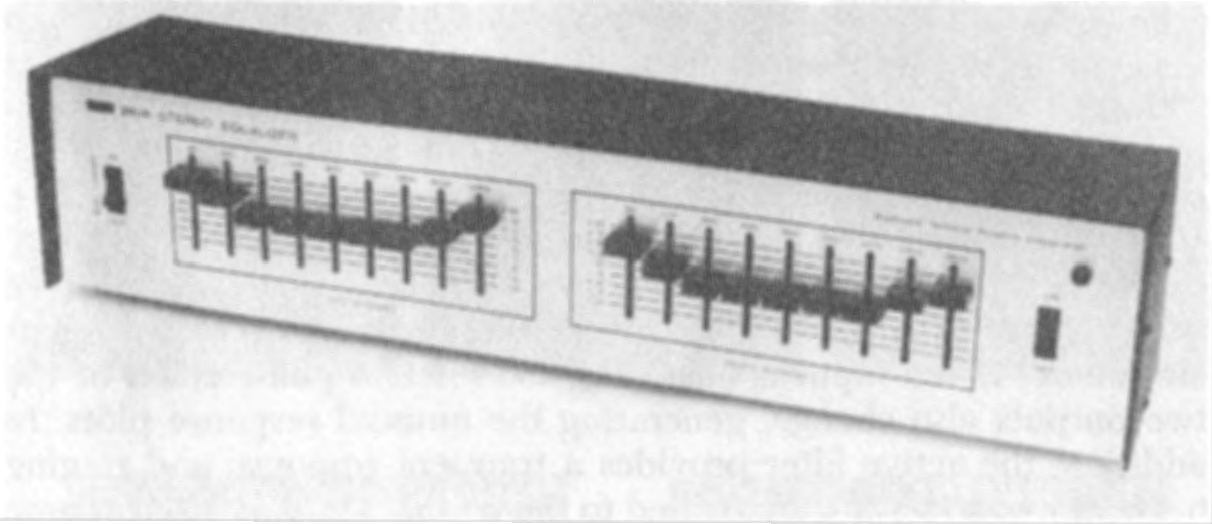
\includegraphics[width=\textwidth]{equalizer}
	\caption{Graphic Equalizer using eighteen active filters}
	\label{fig:equalizer}
\end{figure}
These consist of a bank of slide potentiometers that emphasize or de-emphasize portions of the audio spectrum such that all purpose speakers can be \textit{tuned} to their surrounding environment according to the listener (customer's) preferences. Often, these are made of low-Q, active bandpass filters such as the ones employed here. A sample circuit is shown in Figure \ref{fig:equalizercircuit}.
\begin{figure}[H]
	\centering
	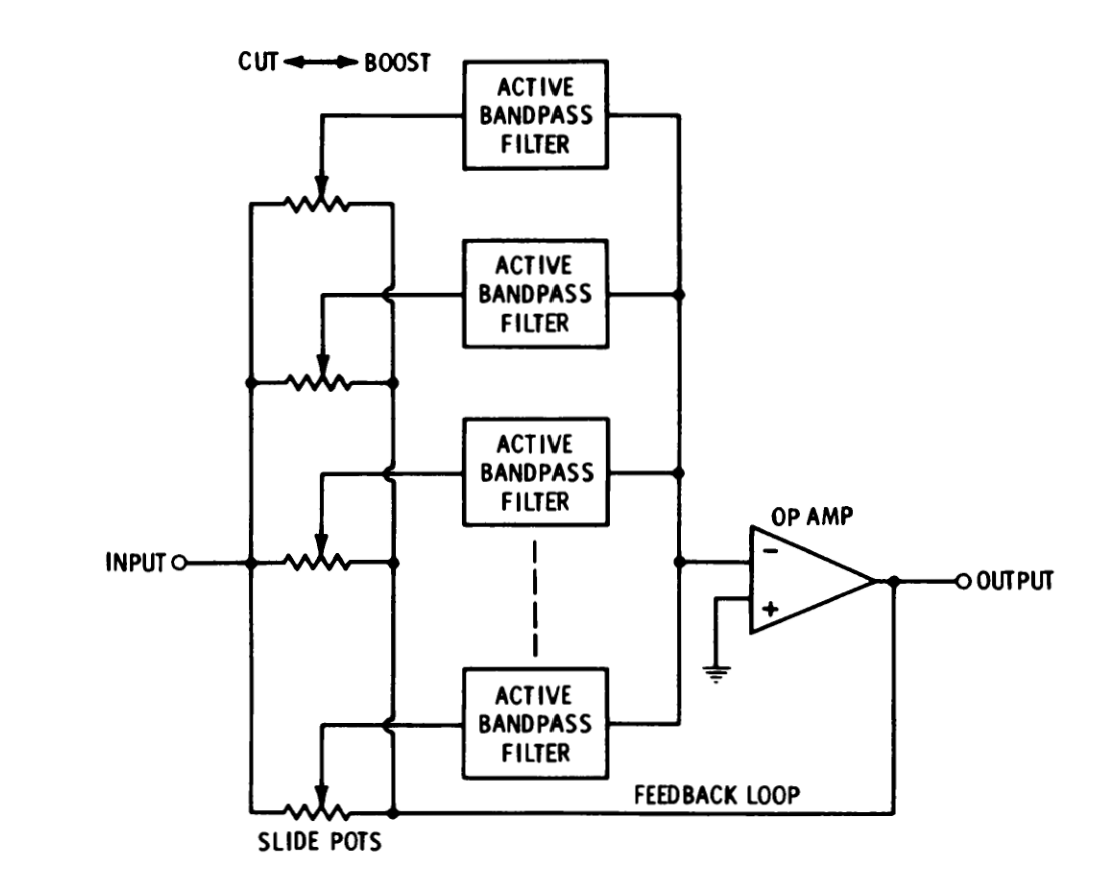
\includegraphics[width=8cm]{equalizercircuit}
	\caption{Graphic Equalizer with Multiple Active Filters in a Loop}
	\label{fig:equalizercircuit}
\end{figure}
These equalizers provide the  ability to ``boost" or ``cut" operation where each slide control provides a flat response in the middle of its range and provide progressively more emphasis or de-emphasis as the limits of the slider are approached.

This design employs some constraints such that the ranges and frequency response is set. A Quality Factor or Q value is also set which determines the slope of the filter at its peaks, or how wide the response is.

\section{Theory}
\subsection{Frequency Range and Q}
With active filters, the useful frequency range is far wider than for any other
filtering technique. The practical lower limit for a filter is somewhere between $0.01$ and $0.1Hz$, where the limiting component is the capacitor size.

The upper limit on frequency is set by the quality of the operational amplifier used. In this case, the $\mu A741$ is used again, which is notoriously out of date. This puts the upper limit in the $100KHz$ to $1MHz$ range. Above these frequencies, the conventional inductor-capacitor filters drop enough in size and cost that they are more practical than operational amplifiers.

When considering Bandpass filters, the narrowness or range of response can also be tuned. This bandwidth of a single filter structure is called its Q and is the ratio of its bandwidth to its center frequency. For example,
\begin{align*}
	f_c & = 200Hz               \\
	f_b & = 2Hz                 \\
	Q   & = \frac{200}{2} = 100
\end{align*}
\subsubsection{Bandwidth}
The bandwidth of a filter is defined as the difference betweeen the upper and lower points of where the filter response finally falls to 3dB below its peak value on the way out of the passband.

\subsubsection{Normalization}
A normalized filter is one such that its component values are adjusted to a convenient frequency and impedance level.

\subsubsection{Cutoff Frequency}
The cutoff frequency is the final point at which the filter response drops by $3 dB$ or approximately $0.707$ of its peak value on the way out of the passband.

\subsection{Multiple-Feedback (MFB) Bandpass Filter}
This project employs the exclusive use of the MFB Bandpass filter in order to tune and achieve the design characteristics. The practical limitations of a single stage MFB are such that the Q of the circuit is limited to quite low Q values.

\begin{figure}[H]
	\centering
	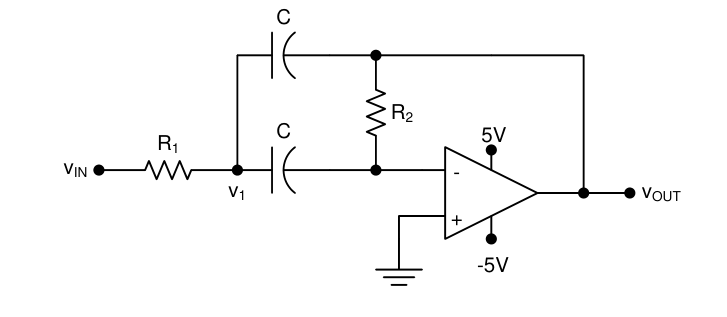
\includegraphics[width=0.75\textwidth]{07_multfeed}
	\caption{Multiple-Feedback Bandpass Filter.}
	\label{fig:multfeed}
\end{figure}

The MFB bandpass filter is another second-order topology but arranges two
resistors and two capacitors in a specific feedback loop. The transfer function can be derived using the node voltage method as such: ($s = j\omega$)
\begin{equation*}
	H(s) \;=\;
	\frac{-sR_2C}
	{s^2R_1R_2C^2 + 2sR_1C + 1}
\end{equation*}

which may be rewritten to match a standard second-order bandpass form:
\begin{align*}
	f_0 & = \frac{1}{2\pi\,C\sqrt{R_1R_2}}    \\
	A_r & = -\frac{R_2}{2R_1}                 \\
	Q   & = \frac{1}{2}\sqrt{\frac{R_2}{R_1}}
\end{align*}
By choosing $R_1$, $R_2$, and $C$, one can specify the center frequency $f_0$ and
quality factor $Q$. Because the peak amplitude occurs at $f_0$, we say the
bandwidth $\mathrm{BW}$ is bounded by the $-3\,\mathrm{dB}$ frequencies, and for
a standard bandpass $Q = \tfrac{f_0}{\mathrm{BW}}$.
\subsection*{Tuning the MFB Bandpass Filter}
Tuning each of the desired frequencies is simply a matter of following Figure \ref{fig:tuning}.

\begin{figure}[H]
	\centering
	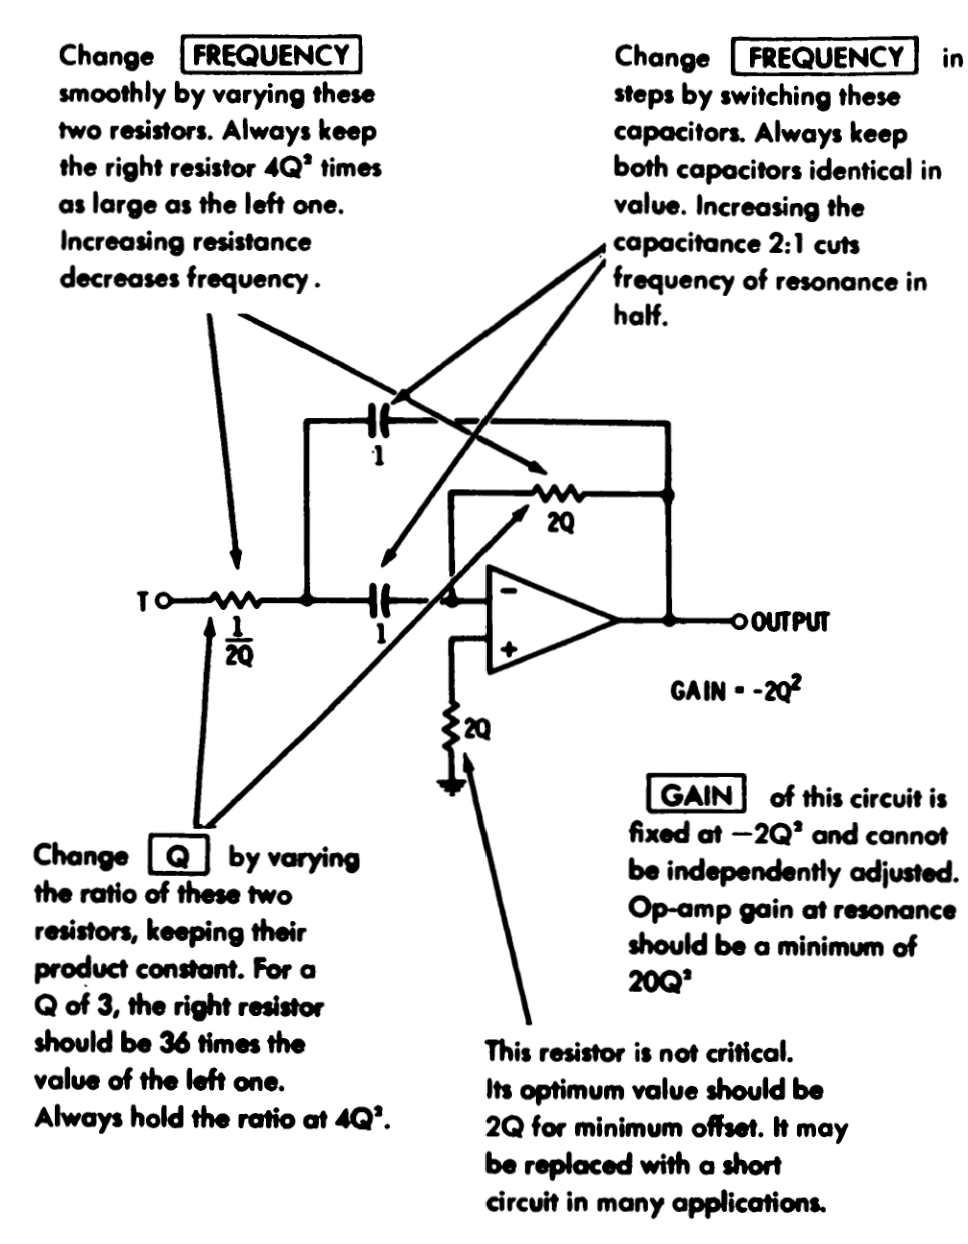
\includegraphics[width=0.5\textwidth]{tuning}
	\caption{Tuning a Multiple-Feedback Bandpass Filter.}
	\label{fig:tuning}
\end{figure}
To begin the tuning and design of the circuit, first the Q factor is considered. Recall,
\[
	Q = \frac{1}{2}\sqrt{\frac{R_2}{R_1}}
\]
All three of the frequency ranges are designed to the same Q of $0.7 \pm 10\%$ or
\[
	1.96 = \frac{R_2}{R_1}
\]

Essentially, this means that as long as the ratio remains constant, the Q will be achieved.
Designing for specifying center frequencies is a matter of choosing a capacitor for the target and then finding a standard resistor ratio that will satisfy it.

To achieve this, the same resistors were used for all three MFB stagess:
\begin{align*}
	R_2 & = 10k\Omega  \\
	R_1 & = 5.1k\Omega
\end{align*}

\subsection{Bass Band}
\noindent \textbf{Specifications:}
\begin{itemize}
	\item Center Frequency - 200Hz
	\item Quality Factor - 0.7
	\item Range of Adjustable Gain 0.4 - 8
\end{itemize}
Utilizing:
\begin{align*}
	f_0 & = \frac{1}{2\pi\,C\sqrt{R_1R_2}}         \\
	200 & = \frac{1}{2\pi\,C\sqrt{5100\cdot10000}} \\
	C   & \approx 110nF                            \\
\end{align*}
\subsection{Midrange Band}
\noindent \textbf{Specifications:}
\begin{itemize}
	\item Center Frequency - 1.0kHz
	\item Quality Factor - 0.7
	\item Range of Adjustable Gain - 0.2 - 4
\end{itemize}
Utilizing:
\begin{align*}
	f_0  & = \frac{1}{2\pi\,C\sqrt{R_1R_2}}         \\
	1000 & = \frac{1}{2\pi\,C\sqrt{5100\cdot10000}} \\
	C    & \approx 22nF                             \\
\end{align*}
\subsection{Treble Band}
\noindent \textbf{Specifications:}
\begin{itemize}
	\item Center Frequency - 5.0kHz
	\item Quality Factor - 0.7
	\item Range of Adjustable Gain 0.1 - 2
\end{itemize}
Utilizing:
\begin{align*}
	f_0  & = \frac{1}{2\pi\,C\sqrt{R_1R_2}}         \\
	5000 & = \frac{1}{2\pi\,C\sqrt{5100\cdot10000}} \\
	C    & \approx 4.7nF                            \\
\end{align*}
The results of this simulated in SPICE can be seen  in Figure \ref{fig:mfbstage}.
\begin{figure}[H]
	\centering
	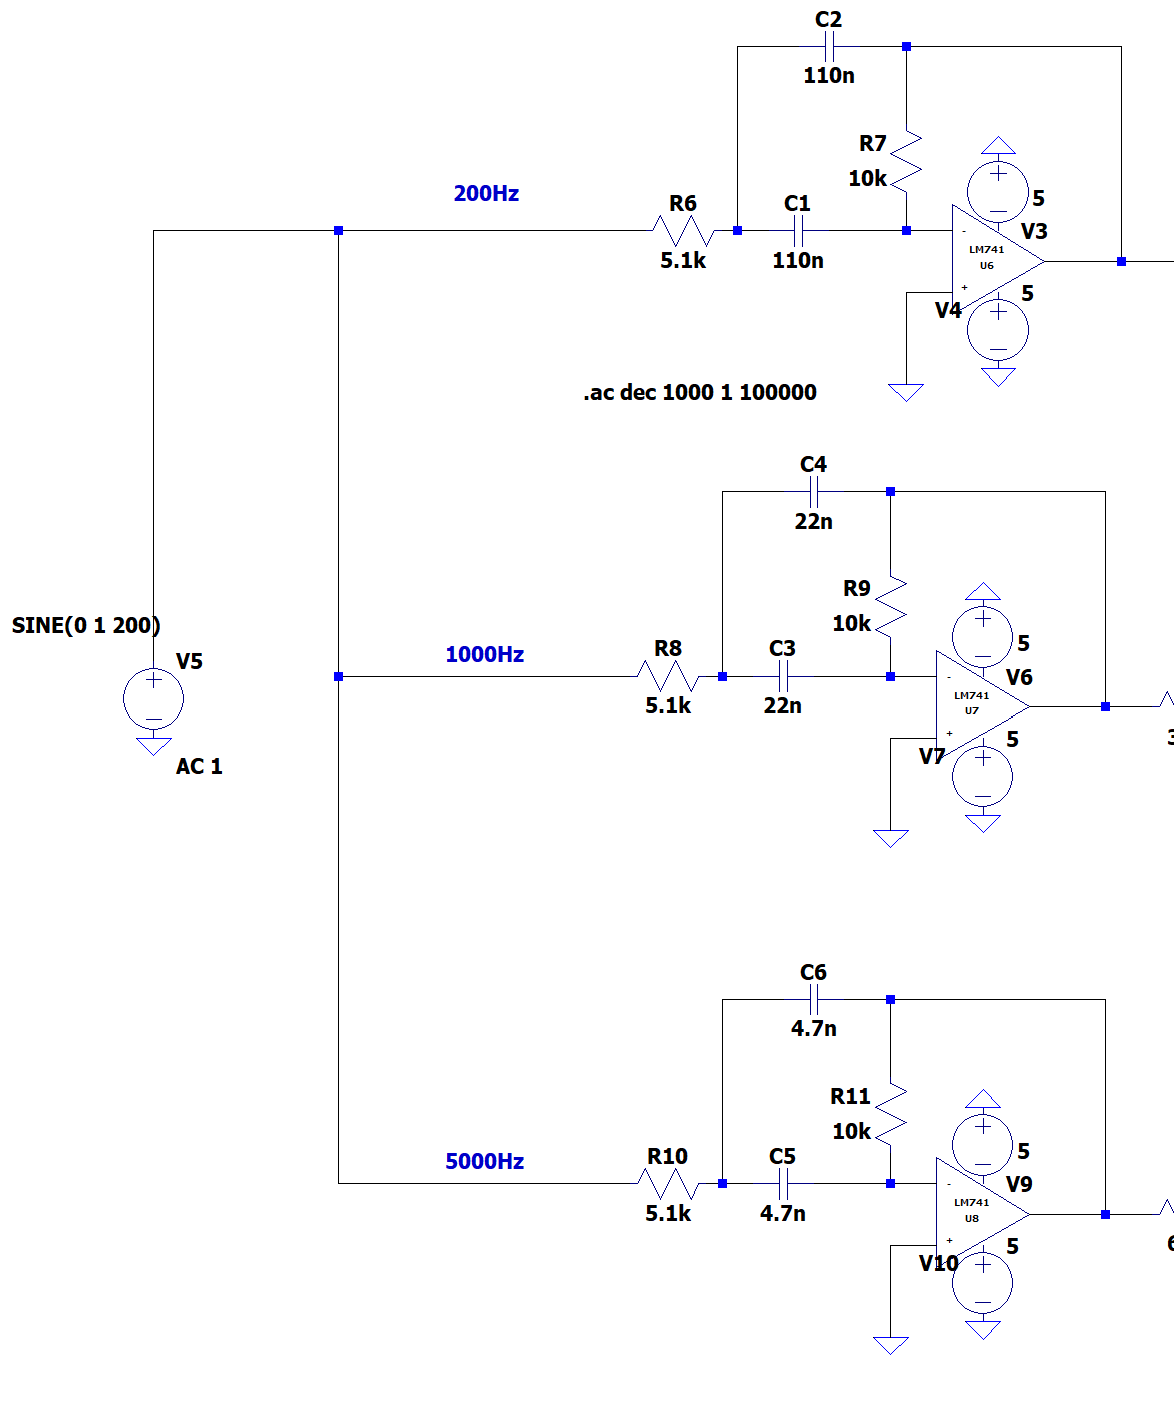
\includegraphics[width=0.8\textwidth]{mfbstage}
	\caption{Frequency Selection Stage}
	\label{fig:mfbstage}
\end{figure}
\section{Gain Control Implementation}

To achieve adjustable gain across the three frequency bands without introducing unnecessary complexity into the filter design, a modular two-stage amplifier system was employed. This approach builds upon techniques developed in a previous design project and allows each frequency band—low, mid, and high—to be individually controlled.

The overall gain structure of the circuit is implemented in two stages:
\begin{itemize}
	\item \textbf{Stage 1: Inverting Summing Amplifier} — Combines the outputs of the three bandpass filters while allowing individual gain control via potentiometers at each input.
	\item \textbf{Stage 2: Post Amplifier} — A single inverting amplifier stage that scales the overall signal amplitude to the desired level using a feedback potentiometer.
\end{itemize}

To allow user-controlled gain adjustments, 10\,k$\Omega$ linear-taper potentiometers were installed in series with each input resistor of the summing amplifier. These were calibrated to achieve the following adjustable gain ranges:
\begin{itemize}
	\item \textbf{Low Frequency Band:} 0.4–8×
	\item \textbf{Midrange Band:} 0.2–4×
	\item \textbf{Treble Band:} 0.1–2×
\end{itemize}

The voltage gain of the inverting summing amplifier is described by the following expression:
\[
	G = -V_1\left(\frac{R_f}{R_1 + x \cdot 10\,\text{k}\Omega}\right)
	-V_2\left(\frac{R_f}{R_2 + y \cdot 10\,\text{k}\Omega}\right)
	-V_3\left(\frac{R_f}{R_3 + z \cdot 10\,\text{k}\Omega}\right)
\]
where:
\begin{itemize}
	\item $V_1$, $V_2$, and $V_3$ are the input voltages from the low, mid, and treble filters respectively,
	\item $R_f$ is the feedback resistor of the summing amplifier,
	\item $R_1$, $R_2$, and $R_3$ are fixed resistors for each input branch,
	\item $x$, $y$, and $z$ are the fractional settings (normalized from 0 to 1) of the potentiometers for each band.
\end{itemize}

Following the summing stage, a post-amplifier was employed to adjust the overall signal level. This stage also used an inverting amplifier topology with a potentiometer in the feedback loop. The voltage gain of this stage is given by:
\[
	G = -\frac{R_f + w \cdot 10\,\text{k}\Omega}{R_{\text{in}}}
\]
where:
\begin{itemize}
	\item $R_f$ is the base resistance in the feedback path,
	\item $w$ is the sweep position of the post-gain potentiometer,
	\item $R_{\text{in}}$ is the input resistor of the inverting amplifier.
\end{itemize}

This design strategy preserves the integrity of the filter characteristics while offering precise, independent, and tunable control over each band's contribution to the output signal. It also simplifies tuning during testing and provides flexibility in adapting the circuit to different listening environments or user preferences.
\section{Experimental Procedures}
\begin{enumerate}
	\item The circuit was simulated in SPICE software
	\item The circuit was built utilizing the theory outlined in the previous section.
	\item The simulation output was compared to the experimental output.
\end{enumerate}

\section{Results and Discussion}

The circuit was tested under three gain configurations—maximum, even, and tuned—each corresponding to specific potentiometer settings targeting different frequency responses. For each configuration, Bode plots were obtained from both LTspice simulations and experimental measurements using Scopy. These results offer valuable insights into the performance, robustness, and limitations of the analog filter system in real-world conditions.

\subsection{Max Value Configuration}

This configuration set the gain maxima to 8 for low, 4 for mid, and 2 for high frequency bands. As shown in Figure~\ref{fig:maxvalue}, the LTspice simulation exhibits well-defined gain peaks aligned with each band's center frequency. The measured response closely tracks the simulation, with only minor attenuation and phase discrepancies.

The high gains used in this setup exposed the effects of parasitic interactions, particularly at high frequencies. The peaking behavior and smooth phase transitions confirm the effectiveness of the filters. Minor deviations are expected due to resistor and capacitor tolerances as well as layout-induced parasitics.

\begin{figure}[H]
	\centering
	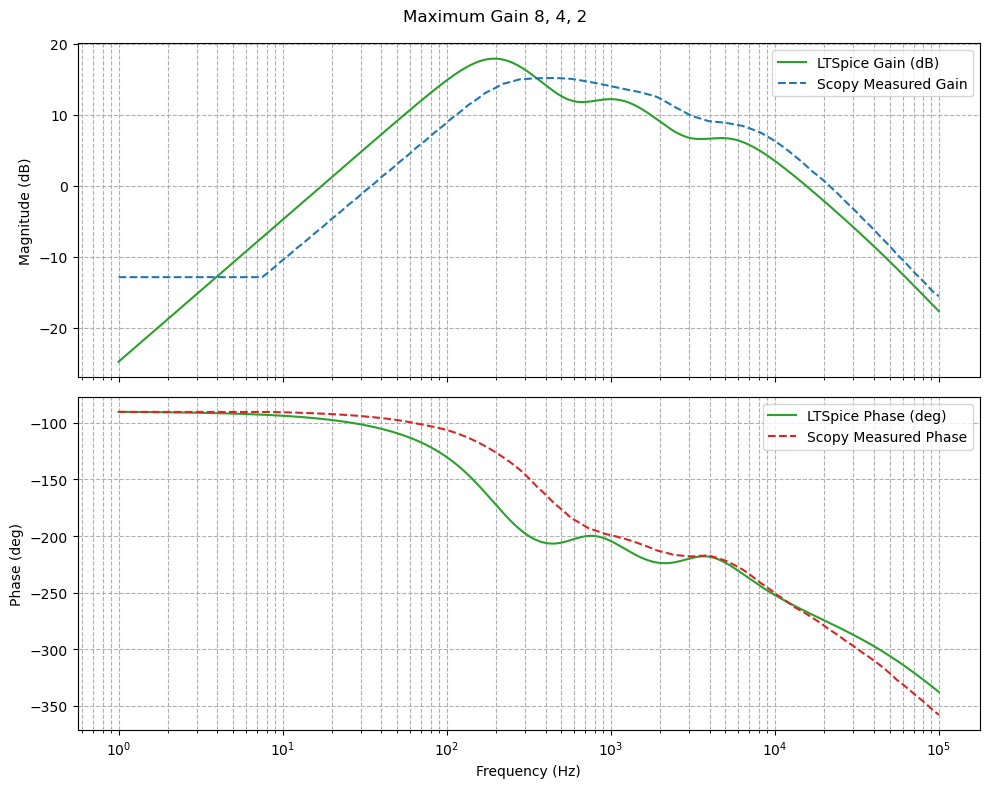
\includegraphics[width=\textwidth]{dp2max.png}
	\caption{Bode plot: Max Gain Configuration (8, 4, 2) — LTspice vs Scopy}
	\label{fig:maxvalue}
\end{figure}
\noindent\textbf{Max Value Gain}
\begin{center}
	\begin{tabular}{|c|c|c|}
		\hline
		\textbf{Freq (Hz)} & \textbf{Gain (dB)} & \textbf{Phase (°)} \\
		\hline
		7.50               & -9.550             & -94.537            \\
		7.50               & -9.550             & -94.537            \\
		19.65              & -1.439             & -96.449            \\
		106.06             & 12.734             & -111.642           \\
		449.88             & 18.497             & -175.126           \\
		1908.29            & 15.822             & 143.065            \\
		10298.60           & 9.397              & 103.891            \\
		43684.00           & -3.807             & 41.802             \\
		235753.00          & -18.683            & -57.598            \\
		1000000.00         & -26.491            & 128.084            \\
		\hline
	\end{tabular}
\end{center}

\subsection{Even Value Configuration}

In this scenario, all bands were configured for uniform gain (2, 2, 2). Figure~\ref{fig:evenvalue} demonstrates strong agreement between simulation and measurement in both gain and phase across a wide frequency range. Compared to the max configuration, the peaks are flatter and more balanced.

The experimental gain trace exhibits slightly less amplification at the midrange peak, possibly due to increased internal resistance in the potentiometer path or measurement bandwidth limits. The phase response remains consistent, validating the correct operation of each filter stage.

\begin{figure}[H]
	\centering
	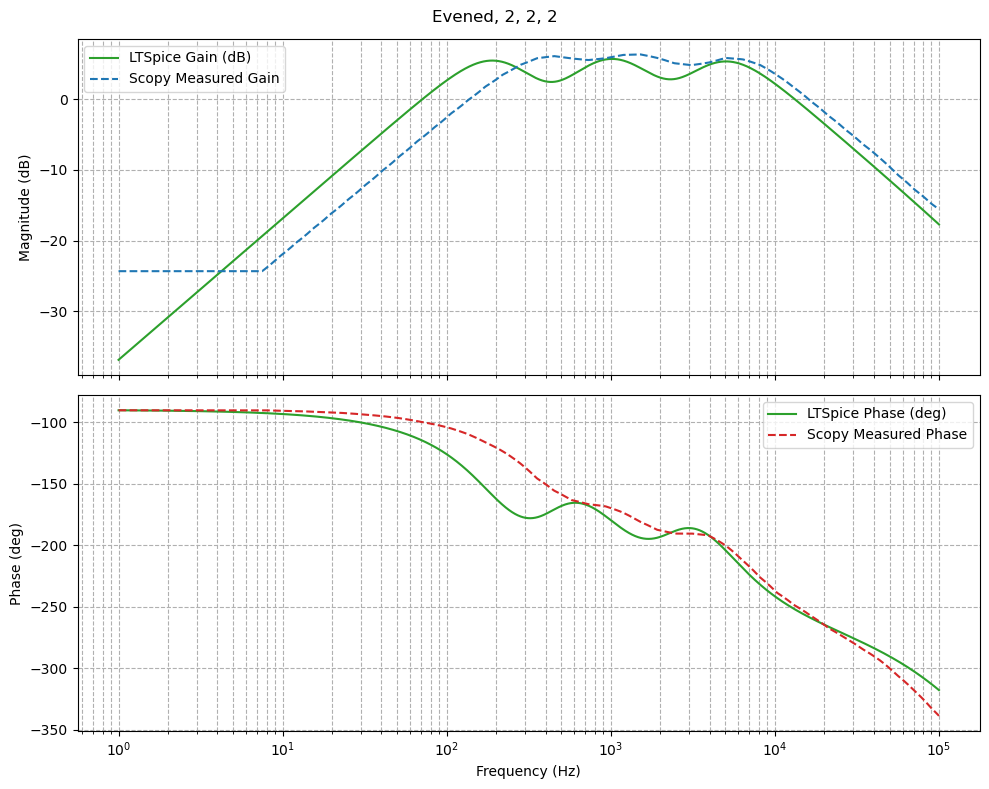
\includegraphics[width=\textwidth]{dp2even.png}
	\caption{Bode plot: Even Gain Configuration (2, 2, 2) — LTspice vs Scopy}
	\label{fig:evenvalue}
\end{figure}

\noindent\textbf{Even Value Gain}
\begin{center}
	\begin{tabular}{|c|c|c|}
		\hline
		\textbf{Freq (Hz)} & \textbf{Gain (dB)} & \textbf{Phase (°)} \\
		\hline
		7.50               & -20.664            & -94.162            \\
		7.50               & -20.664            & -94.162            \\
		19.65              & -12.556            & -95.822            \\
		106.06             & 1.614              & -108.884           \\
		449.88             & 9.736              & -159.395           \\
		1908.29            & 9.490              & 168.726            \\
		10298.60           & 7.037              & 117.515            \\
		43684.00           & -4.699             & 62.514             \\
		235753.00          & -18.096            & -46.562            \\
		1000000.00         & -26.585            & 127.592            \\
		\hline
	\end{tabular}
\end{center}

\subsection{Tuned Configuration}

The tuned configuration targeted realistic application-specific gains: 0.4, 0.8, and 1.6 for low, mid, and high bands respectively. Figure~\ref{fig:tunedvalue} shows remarkably close tracking between LTspice and Scopy gain responses, especially in the mid-to-high frequency ranges.

At very low frequencies, however, slight discrepancies were observed. These may be attributed to capacitor tolerances, breadboard leakage, or coupling with the protoboard’s internal capacitance, which can disproportionately affect small-value capacitors. Despite this, the circuit exhibits expected gain shaping and continuous phase rotation, indicating proper filter engagement and summing behavior.

\begin{figure}[H]
	\centering
	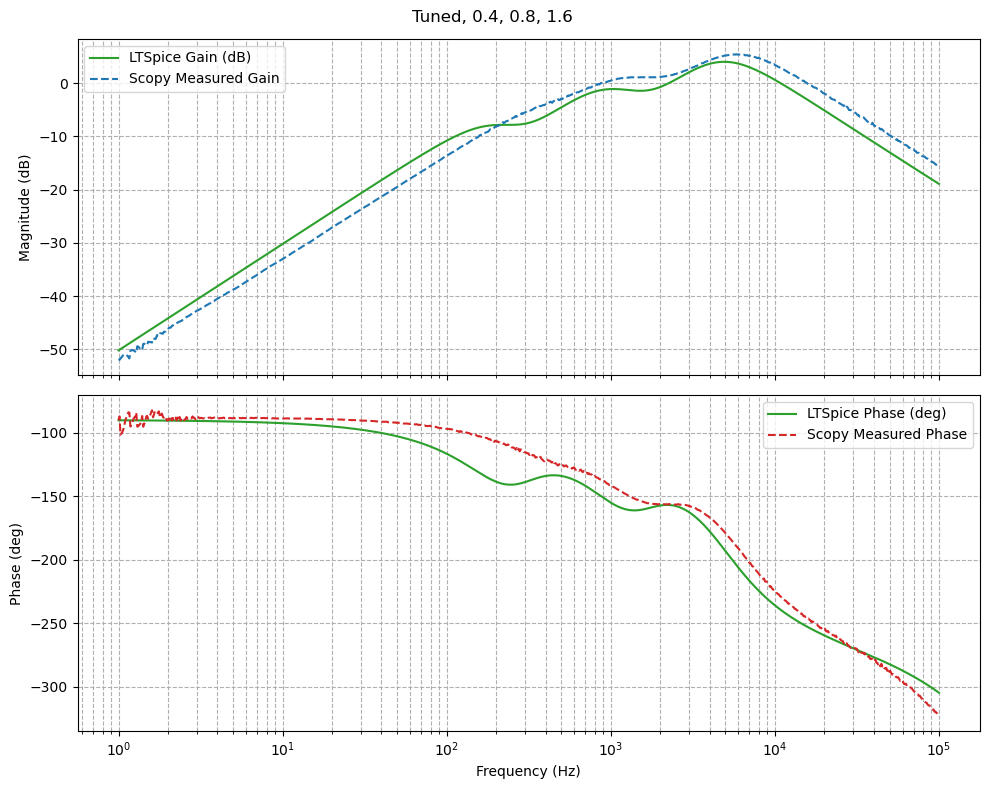
\includegraphics[width=\textwidth]{dp2tuned.png}
	\caption{Bode plot: Tuned Gain Configuration (0.4, 0.8, 1.6) — LTspice vs Scopy}
	\label{fig:tunedvalue}
\end{figure}

\noindent\textbf{Tuned Value Gain}
\begin{center}
	\begin{tabular}{|c|c|c|}
		\hline
		\textbf{Freq (Hz)} & \textbf{Gain (dB)} & \textbf{Phase (°)} \\
		\hline
		1.00               & -49.963            & -95.851            \\
		4.64               & -37.468            & -93.721            \\
		21.54              & -24.633            & -95.180            \\
		100.00             & -11.793            & -102.618           \\
		464.16             & -1.433             & -129.927           \\
		2154.43            & 3.185              & -161.996           \\
		10000.00           & 5.245              & 129.874            \\
		46415.90           & -7.228             & 69.091             \\
		215443.00          & -19.827            & -26.199            \\
		1000000.00         & -28.952            & 125.331            \\
		\hline
	\end{tabular}
\end{center}
\section{Conclusion}

The experimental results closely corroborated the simulated data, validating the circuit design and underlying gain calculations. Each configuration exhibited expected frequency shaping and phase shift behaviors. The peaking observed in both simulation and measurement demonstrates the correct operation of the bandpass filters.

Some deviations in gain magnitude were noted between Scopy and LTspice results. These are most likely attributed to:
\begin{itemize}
	\item Component tolerances (especially capacitors in the pF range),
	\item Breadboard parasitic capacitance,
	\item External electromagnetic interference,
	\item Limited frequency resolution or dynamic range in the measurement setup.
\end{itemize}

Despite these real-world imperfections, the system demonstrated predictable behavior and strong agreement with theoretical expectations. The ability to independently tune the gain of each band proved highly effective and practical, reinforcing the utility of the modular summing and post-amplifier architecture.
\end{document}
% vim: set ft=tex tw=80 ts=2 sts=2 sw=2 noet spell:
